\documentclass[UTF8]{ctexart}

\usepackage{amsmath}
\usepackage{cases}
\usepackage{cite}
\usepackage{graphicx}
\usepackage{booktabs}
\usepackage{verbatim}
\usepackage{bm}
\usepackage[margin=1in]{geometry}
\usepackage{pifont} %ding{172}\ding{173}\ding{174}\ding{175}\ding{176}\ding{177}\ding{178}\ding{179}\ding{180}\ding{181}
\geometry{a4paper}
\usepackage{multirow} 
\usepackage{fancyhdr}
\usepackage{diagbox}
\usepackage{subfigure}
\usepackage{listings}
\usepackage{float}
\pagestyle{fancy}
\fancyhf{}
\title{REDC3329\_pipeline设计文档}
\author{李远政 U202211014}
\date{2025年9月}
\pagenumbering{arabic}
\begin{document}
	\maketitle
	\tableofcontents
	\newpage
	\fancyhead[L]{李远政}
	\fancyhead[C]{REDC3329\_pipeline设计文档}
	\fancyhead[R]{2025.9}
	\fancyfoot[C]{\thepage}
	\section{模块要求}
根据任务要求实现一个12-bit位宽的流水线快速模乘器模块。模乘器输入a、b两个12-bit位宽的乘数,给定模数q=3329,在固定周期内输出a*b mod q。要求当模乘器输入使能有效时,a、b两个乘数输入,随后模乘器进行计算,在模乘器计算过程中,busy信号指示高电平为忙状态,否则为低电平指示空闲状态。在经过固定周期后,done信号由低变高,指示计算完成,同时输出结果。
	\section{模块输入输出说明}

	\begin{table}[h!]
		\begin{center}
			\caption{IO接口表}
			\setlength{\tabcolsep}{2pt}
			\begin{tabular}{c c c c}
\toprule
        \textbf{端口} & \textbf{方向} & \textbf{位宽} & \textbf{描述} \\
        \midrule
        \texttt{clk}   & Input  & 1  & 系统时钟信号。 \\
        \texttt{rst\_n} & Input  & 1  & 低电平有效的异步复位信号。 \\
        \texttt{en}    & Input  & 1  & 使能信号。当 \texttt{en} 为高时,模块在下一个时钟周期锁存输入 \texttt{a} 和 \texttt{b}。 \\
        \texttt{a}     & Input  & 12 & 输入操作数 A。 \\
        \texttt{b}     & Input  & 12 & 输入操作数 B。 \\
        \texttt{busy}  & Output & 1  & 忙信号。当模块正在处理数据时(从 \texttt{en} 拉高到 \texttt{done} 拉高之间),该信号为高。 \\
        \texttt{done}  & Output & 1  & 完成信号。当一次模乘计算完成,且输出 \texttt{r} 有效时,该信号拉高一个时钟周期。 \\
        \texttt{r}     & Output & 12 & 计算结果,即 \texttt{(a * b) mod 3329}。 \\
        \bottomrule
			\end{tabular}
		\end{center}
	\end{table}
	\section{算法理论与算法验证}
	\subsection{Montgomery模乘算法}
可以观察到题目中所给出的3329是一个质数,所以可以使用蒙哥马利算法简化取模的计算过程。算法的基本原理是通过一系列的转换将本来对一个普通数N的取模转换为对一个2的幂次R的取模过程,从而可以通过移位算法节省大量计算资源。为了达到对一个数T转换模数的目的,先构造REDC(a,b,R)函数解决$(ab)\cdot R^{-1} (mod N)$的问题,这个函数是存在简便算法的。然后反复调用这个函数来实现模乘的过程。具体步骤如下:
\subsubsection{REDC函数的设计}
构造函数的基本思路是将大数T加上一个适当的数值m,使其能够被R整除,并且结果能够落在0到2N的范围内,并且仍然保证对N同余的特性。这样就可以直接使用简单的数据选择器实现对于N的取模。具体步骤如下:
首先构造加数:
$$
m=N[T(mod R)N^\prime](modR)
$$
其中:
$$
N\cdot N^\prime=-1(mod R)
$$
相加之后得到t:
$$
t=T+m=T+N[T(mod R)N^\prime](modR)=T+[(NN^\prime)(modR)][(T(mod R))](modR)=T-T(modR)
$$
将t再modR的情况下进行化简:
$$
t(modR)=T+[(NN^\prime)(modR)][(T(mod R))](modR)=T-T(modR)
$$
从上面的变换中,不难看出这个t是可以被R整除的。接下来将t除以R得到:
$$
u=\frac{T+m}{R}
$$
现在来估算u的范围:
$$
T<N\cdot R
$$
$$
N[T(mod R)N^\prime](modR)<N\cdot R
$$
$$
 0\leq t<2N
$$
因此可以直接通过比较t和N的大小来实现对N的取模。
\subsubsection{REDC函数的乘法性质}
因为直接调用REDC函数会带有R的逆元,无法直接得到结果,所以通过多次调用转换来实现模乘的过程。具体步骤如下:\\
1.转换输入a,b为蒙哥马利域下的数:
$$
a_{mont}=REDC(a,R^2)
$$
$$
b_{mont}=REDC(b,R^2)
$$
2.计算a,b的乘积:
$$
t=REDC(a_{mont},b_{mont})
$$
3.将结果转换回普通域下的数:
$$
r=REDC(t,1)
$$
这样就刚好通过两部约去了最开始引入的R的次方影响,得到了正确的结果。
\section{电路设计}
\subsection{REDC3329整体架构}
整体结构在计算部分采用流水线的设计按照设计原理的要求分为三个阶段,分别是输入转换阶段,乘法计算阶段,输出转换阶段。每个阶段都使用寄存器锁存数据,并且通过控制逻辑实现各个阶段的流水线操作。具体结构如下图所示:
\begin{figure}[H]
	\centering
	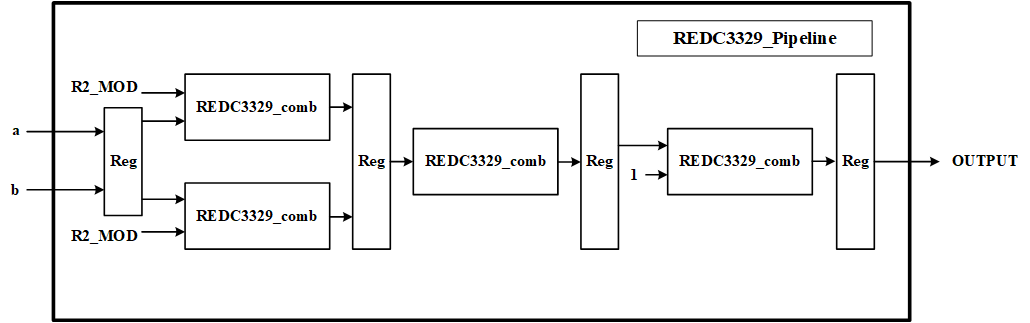
\includegraphics[scale=0.65]{1.png}
	\caption{流水线模乘器结构图}	
\end{figure}
\subsection{REDC模块设计}
REDC模块的设计是整个模乘器的核心部分,主要负责实现蒙哥马利模乘算法中的REDC函数。该模块接受一个24-bit的输入T,并输出一个12-bit的结果r,同时还需要处理一些中间变量和状态信号。具体设计如下:
\begin{figure}[H]
	\centering
	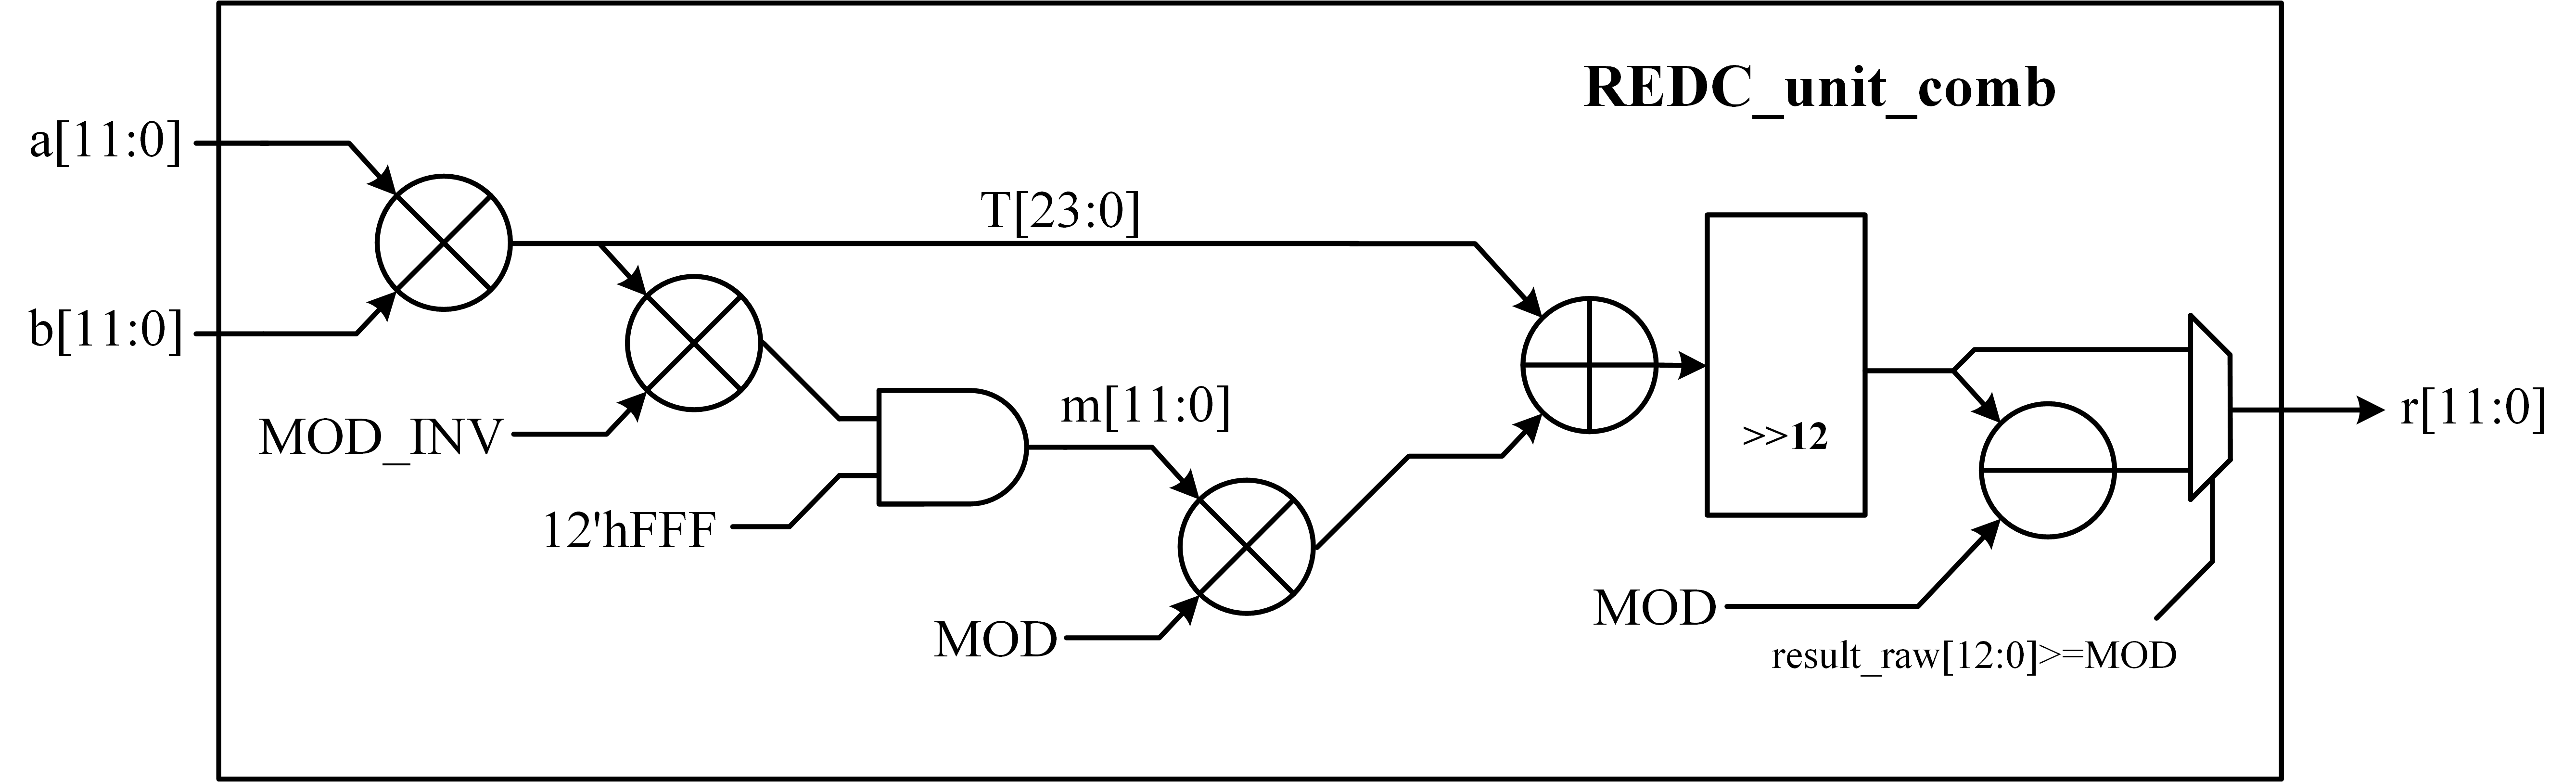
\includegraphics[scale=1.2]{2.png}
	\caption{REDC3329\_unit\_comb结构图}	
\end{figure}
\section{功能验证}
\subsection{仿真验证}
因为12bit输入范围较小,可以通过穷举所有输入的方式来验证设计的正确性。编写了一个简单的testbench来实
现该功能。将theroy信号进行四个周期的打拍,然后和r进行对比,如果不相等则说明设计有误。为了方便观测结果,在仿真平台中添加wrong信号,将两个信号进行异或,如果出现错误的计算结果可以直接观测到wrong信号置1。仿真结果显示在所有的12-bit位宽输入下,wrong信号在复位完成之后的计算过程中始终为低电平,说明设计的结果和理论结果完全一致,验证了设计的正确性。
\begin{figure}[H]
	\centering
	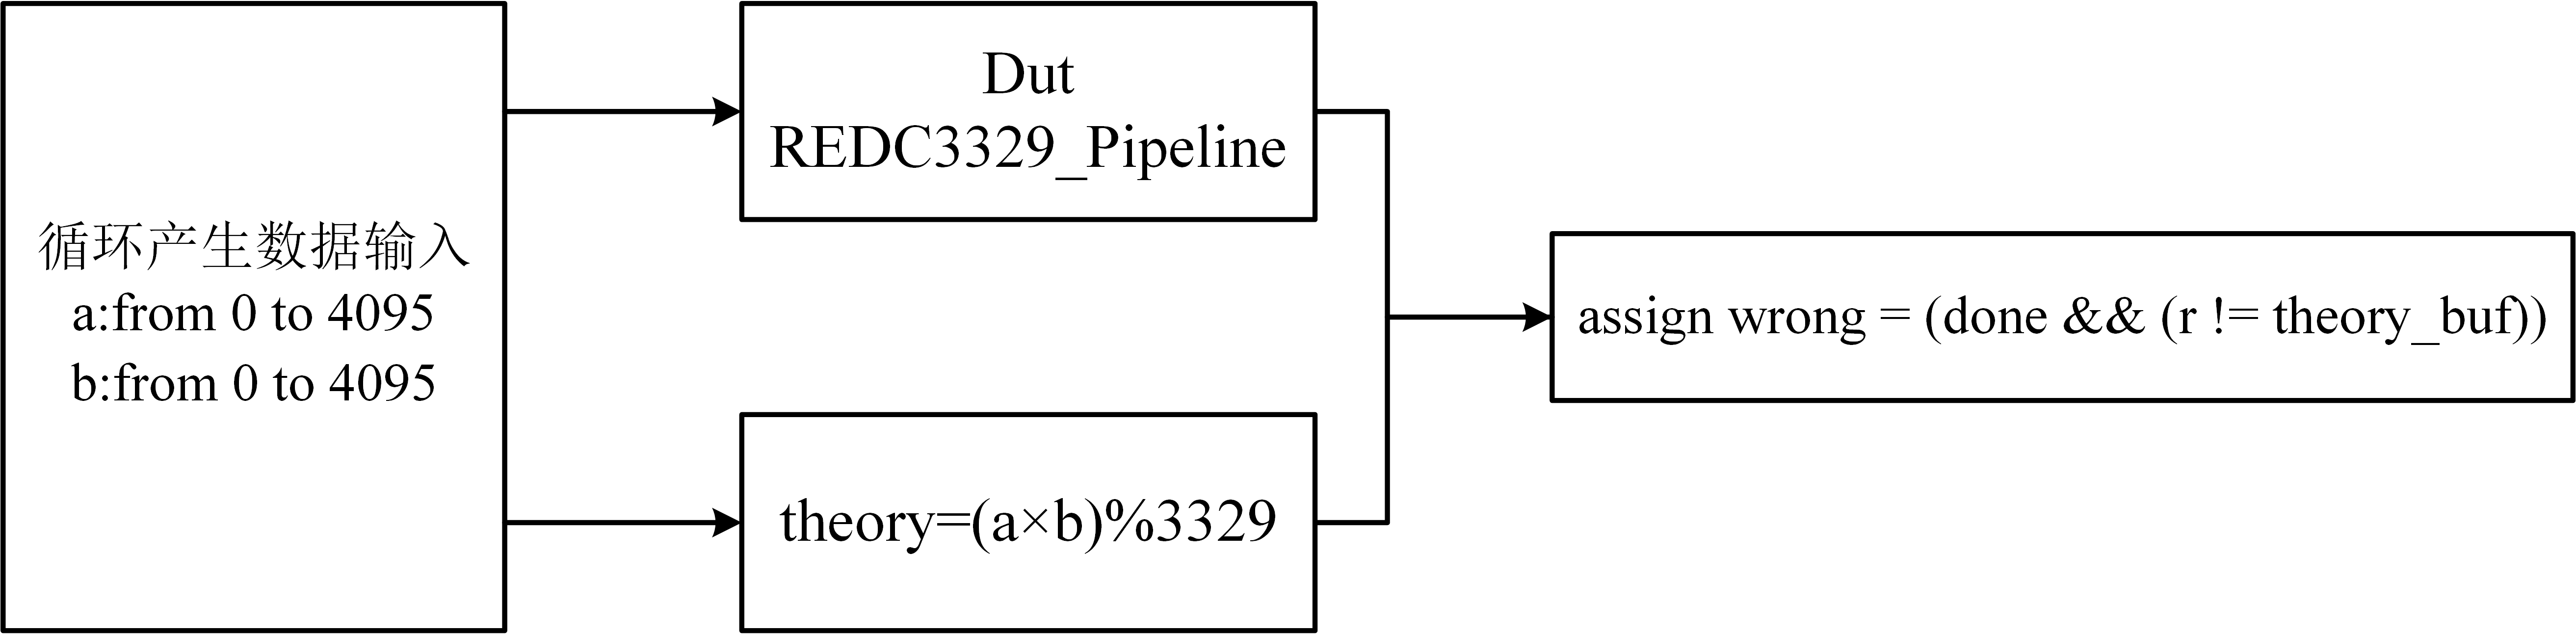
\includegraphics[scale=1.2]{sim.png}
	\caption{仿真流程设计图}	
\end{figure}
\begin{figure}[H]
	\centering
	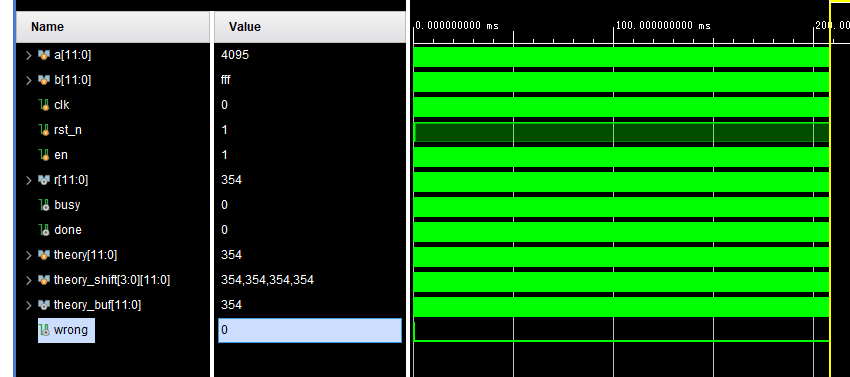
\includegraphics[scale=0.7]{wrong.png}
	\caption{仿真波形图}	
\end{figure}
\subsection{综合实现}
	设置实现约束文件指定时钟周期为20ns,暂不考虑外设时序问题。
	\par 使用ZYNQ-7020作为芯片型号经过综合和实现之后,最终的时序报告显示在该时钟周期下没有违反时序的情况。资源利用率方面,整体设计使用了较少的逻辑单元和寄存器资源,具体资源利用率如下表所示:
\begin{figure}[H]
	\centering
	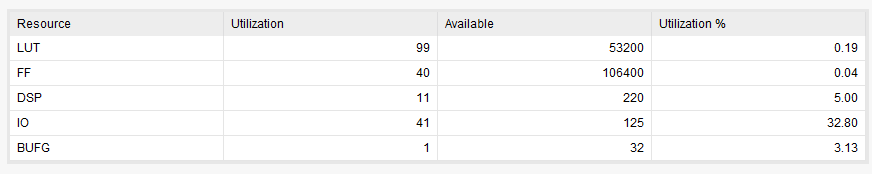
\includegraphics[scale=0.7]{usage.png}
	\caption{资源占用统计}	
\end{figure}
\begin{figure}[H]
	\centering
	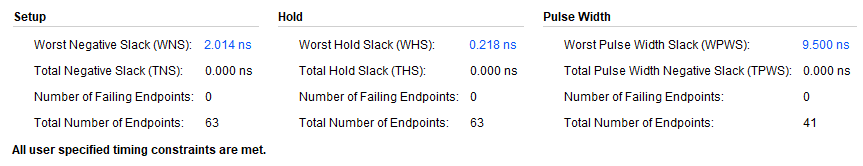
\includegraphics[scale=0.7]{timming.png}
	\caption{时序报告}	
\end{figure}
\begin{figure}[H]
	\centering
	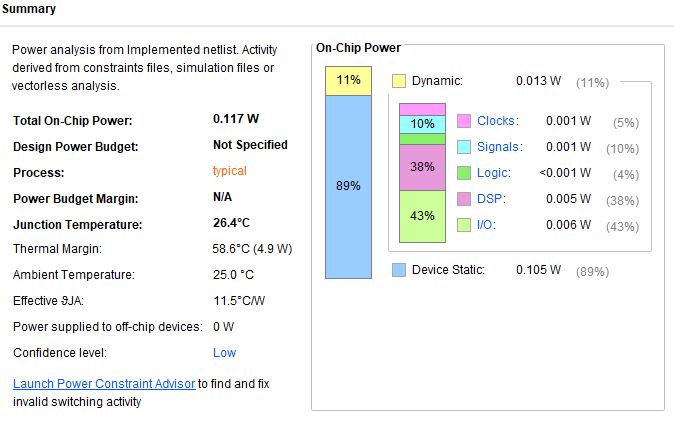
\includegraphics[scale=0.7]{power.png}
	\caption{功耗报告}	
\end{figure}
	\begin{comment}

	\textsuperscript{\footnotesize\cite{shitailong}}


	\begin{thebibliography}{99}
\bibitem{shitailong}


\begin{thebibliography}{99}
\bibitem{shitailong}
史泰龙. 胶体量子点短波红外探测器的器件物理研究[D]. 湖北:华中科技大学,2021.
\bibitem{zongshu1}
马润泽,张晓明,冯帅,等.红外光电探测技术研究现状及展望(特邀)[J].光子学报,2021,50(10):1004006
\bibitem{zongshu2}
李汝劼,唐利斌,张玉平,赵清.红外量子点及其光电探测器研究进展[J].红外技术,2020,42(5):405-419
\bibitem{art1}
Tiande Liu.Room-temperature infrared photodetectors with hybrid structure based on two-dimensional materials[J].《Chinese Physics B》,2019
\bibitem{art2}
尉鹏举.InAs/GaSbⅡ类超晶格多色红外探测器降低串音影响的研究进展[J].《真空与低温》,2025
\end{thebibliography}


史泰龙. 胶体量子点短波红外探测器的器件物理研究[D]. 湖北:华中科技大学,2021.

\end{thebibliography}
\begin{figure}[h]
	\centering
	\includegraphics[scale=0.5]{sbq2.png}
	\caption{DIRS=1正向循环仿真}	
\end{figure}

\begin{itemize}
		\item 在线上实习中学习了反相器制作工艺的相关知识。
		\item 在线上实习中体验了光刻工艺的全流程,了解了光刻工艺的基本原理和步骤。
		\item 在线下实习中参与了与量子点红外芯片成像相关的讲座,了解了量子点红外芯片的基本原理和应用。
		\item 走进了实验室,学习了PbS CQD 红外探测器的制备的部分工艺步骤。
		\item 自主对相关前沿知识进行了学习。
	\end{itemize}

	\begin{table}[h!]
		\begin{center}
			\caption{实验所需的元器件}
			\setlength{\tabcolsep}{20pt}
			\begin{tabular}{c c c}
				\toprule
				\textbf {名称} & \textbf {型号(参数)} & \textbf {数量}\\
				\midrule
				\textbf{FPGA开发板} 	&  Digilentt Basys2 & 1片\\
				%\hline
				\bottomrule
			\end{tabular}
		\end{center}
	\end{table}

	(Get-Content .\数电实验1.tex | Measure-Object -Character).Characters



		\end{comment}
\end{document}